\section{引言}
电子和传感器技术的进步拓宽了无人机的应用范围~\cite{bekmezci2013flying, bok2011context}包括但不限于交通监控、野外救援、商业快递和遥感等方面。
由于飞行场景的复杂性和不可控性,大多数飞行控制程序(如:\tool{PX4}~\cite{px4}、\tool{LibrePilot}~\cite{Librepilot}和\tool{ArduPilot}~\cite{ardupilot})都实现了一种动态调整机制,即参数配置。
这种参数配置机制可以让使用者或者开发者根据自身需求来平衡无人机的的可靠性(保持稳定飞行)和适应性(适用于更多场景)。
这种参数配置机制提供了大量的可调整参数来适应飞行硬件和任务的差异,例如可以调整无人机飞行的姿态的增益参数,电机的最大转速,任务飞行允许最大的倾角。
一个可靠而灵活的控制程序包含了数百个影响飞行行为的飞行参数。

然而,这些配置的安全性是不可预测的,因此在没有提前飞行测试的情况下,一些不适当的配置可能会被上传到无人机中,从而导致无人机做出不可逆的不稳定飞行。
例如,它会造成无人机实际的飞行轨迹偏离其预先规划的路径从而导致轨迹偏离,或者由于姿态异常导致电机无法提供更多的动力来维持飞行并进一步出现飞行推力损失警告,甚至这些配置可能会直接导致无人机坠毁。
为了维护配置的安全性和可靠性,控制程序的开发者或制造商提供了参数值选择的建议范围,以防止像这些不稳定的飞行那样的不可预测的事件发生。
虽然开发者在上尝试在安全配置方面做出了一定的防御机制,但由于缺乏对参数值的充分检查,这种范围限制机制仍然暴露出\textit{范围规范错误(Range Specification Bugs})。
具体来说,即使一些特定的配置中的参数值均在范围建议内,仍然可能被触发一些不稳定的飞行,即官方建议不能防止配置驱动无人机进入不稳定的飞行。

不幸的是,现有的无人机漏洞检测技术并不以检测/搜索这种漏洞为目的。
污点分析~\cite{cheng2018dtaint, she2020neutaint, chibotaru2019scalable, halin2019test}跟踪参数数据流以定位它对系统的影响。
然而,当处理非常多的控制参数时,每个参数都有很大的取值范围,测试覆盖所有的值是很耗时的。
此外,这种跟踪是在程序运行时进行的,这意味着对问题的定位需要进行无人机飞行任务测试来完成。
相关先进研究\tool{RVFuzzing}~\cite{rvfuzzer}使用模糊测试的方法来发现这种配置从而解决这样的问题。
尽管\tool{RVFuzzing}提出了两种二进制搜索方法来模糊测试配置的数量,但它仍然无法实现高覆盖率,并错过了一些包含不正确配置的搜索空间。
\tool{LGDFuzzer}~\cite{han2022control}采用了一种带有学习模型的模糊测试来评估配置,以加速搜索过程。
然而,该工作中的评估只考虑一个时间戳的预测偏差,这使得搜索结果很可能受到瞬时干扰的影响,影响搜索的准确性。

本章节提出一种新的基于模型预测的可靠参数配置方案,并实现了原型工具\icsearcher,一种带有预测器的模糊方法,它能够搜索不正确的配置并提供较为合理的范围指导以减少\textit{范围实现错误}出现的可能性。
整体上讲,\icsearcher 依赖于遗传算法(Genetic Algorithm,GA)~\cite{ga}和飞行状态预测器来检测潜在的不正确配置并从范围指南中剔除。 
具体来说,\icsearcher 由三个模块组成,即参考状态预测器、不正确搜索器和灵活的范围指南。
该方案首先通过手动收集飞行日志来创建生成预测器所需的数据,数据中的每个条目都包含飞行状态、传感器数据、配置和时间戳。
随后,\icsearcher 使用这些数据生成一个预测器,并使用它来估计一段一个无人机飞行的下一时刻的参考状态。
\icsearcher 的核心在于使用GA进行模糊搜索,从而找到潜在的不正确配置,这些配置被预测器评估为可能会导致无人机不稳定。
与传统的模糊验证方案,即通过现实或模拟执行来测试候选者不同,\icsearcher 用该预测器替代了GA中的反馈评估,即使用概率预测结果来驱动模糊搜索。
最后,\icsearcher 验证了被预测为\dquote{不正确}的配置,并根据这些验证结果进一步生成了灵活的参数范围。

\section{参数范围实现错误}
制造商提供由数百个参数组成的可配置控制方案,以支持各种飞行任务。
每个用户或者控制端可以通过调整这些参数值来控制无人机,以应对不同的任务场景。
然而,一些数值组合可能会导致不稳定的状态。
因此,控制系统的制造商同时提供了一种范围控制机制,通过每个参数的预设值范围指导参数选择。
以前的研究表明,这样的范围控制机制不能防止引入不正确的配置,即使是从预设范围内选择有效的参数值。
这些不正确的配置所造成的问题被称为\textit{范围规范错误(Range Specification Bugs)}~\cite{rvfuzzer, han2022control}。
这些配置会导致不稳定的飞行状态,并可能导致轨迹偏差和坠机等严重事故。
范围规范的错误从两个方面威胁着无人机,即外部攻击和内部误配置(如图~\ref{fig:range_attack}所示)。
\begin{itemize}

 \item \textbf{内部误配置:}
无人机的管理人员或内部人员,不熟悉配置无人机的正确方法,错误地配置了不适当的参数值。
不正确的配置会导致异常的飞行预期,由于缺乏准备知识,用户无法确定问题的根本原因。

\item \textbf{外部攻击:}假设攻击者通过模拟测试模拟无效的配置,可以利用无线/无线电通信的漏洞~\cite{kwon2018empirical,rodday2016exploring, vanhoef2017key}。
在没有任何恶意代码注入、内存损坏或传感器欺骗的情况下,攻击者构建并通过脆弱的无线/无线电通道向无人机发送了一连串的命令。
通过秘密地不正确的些配置发送给无人机,从而触发不稳定的物理状态并中断飞行任务。
为什么攻击者要费心去修改配置,而不是直接让无人机崩溃呢?
一个关键的考虑因素是这些攻击侧重于利用协议中的漏洞,而不是针对飞行系统,这意味着它们可以在不依赖代码注入或固件修改的情况下实现其目标。
需要注意的是,由于没有物理接触,攻击者无法轻易通过操纵控制程序来破坏或控制无人机。 
相反,这些协议充当用户和无人机之间的主要通信渠道,使它们成为潜在攻击的主要入口点。
与常规的用于进行攻击的恶意命令不同的是,不正确配置攻击利用的是无人机系统自身的逻辑设计缺陷而不是外部系统入侵。
而最近的研究~\cite{schiller2023drone}使用协议反向的方法将无人机的内部命令发送给DJI无人机,从而导致无人机重新连接。
这凸显了伪造命令和利用系统中的逻辑漏洞(例如范围规范错误)可能是攻击者的有效方法。 此外,此类攻击的优点是利用本机机制掩盖攻击者的意图,从而可能混淆后续的事故调查。



\end{itemize}

\begin{figure}[ht]
  \centering
    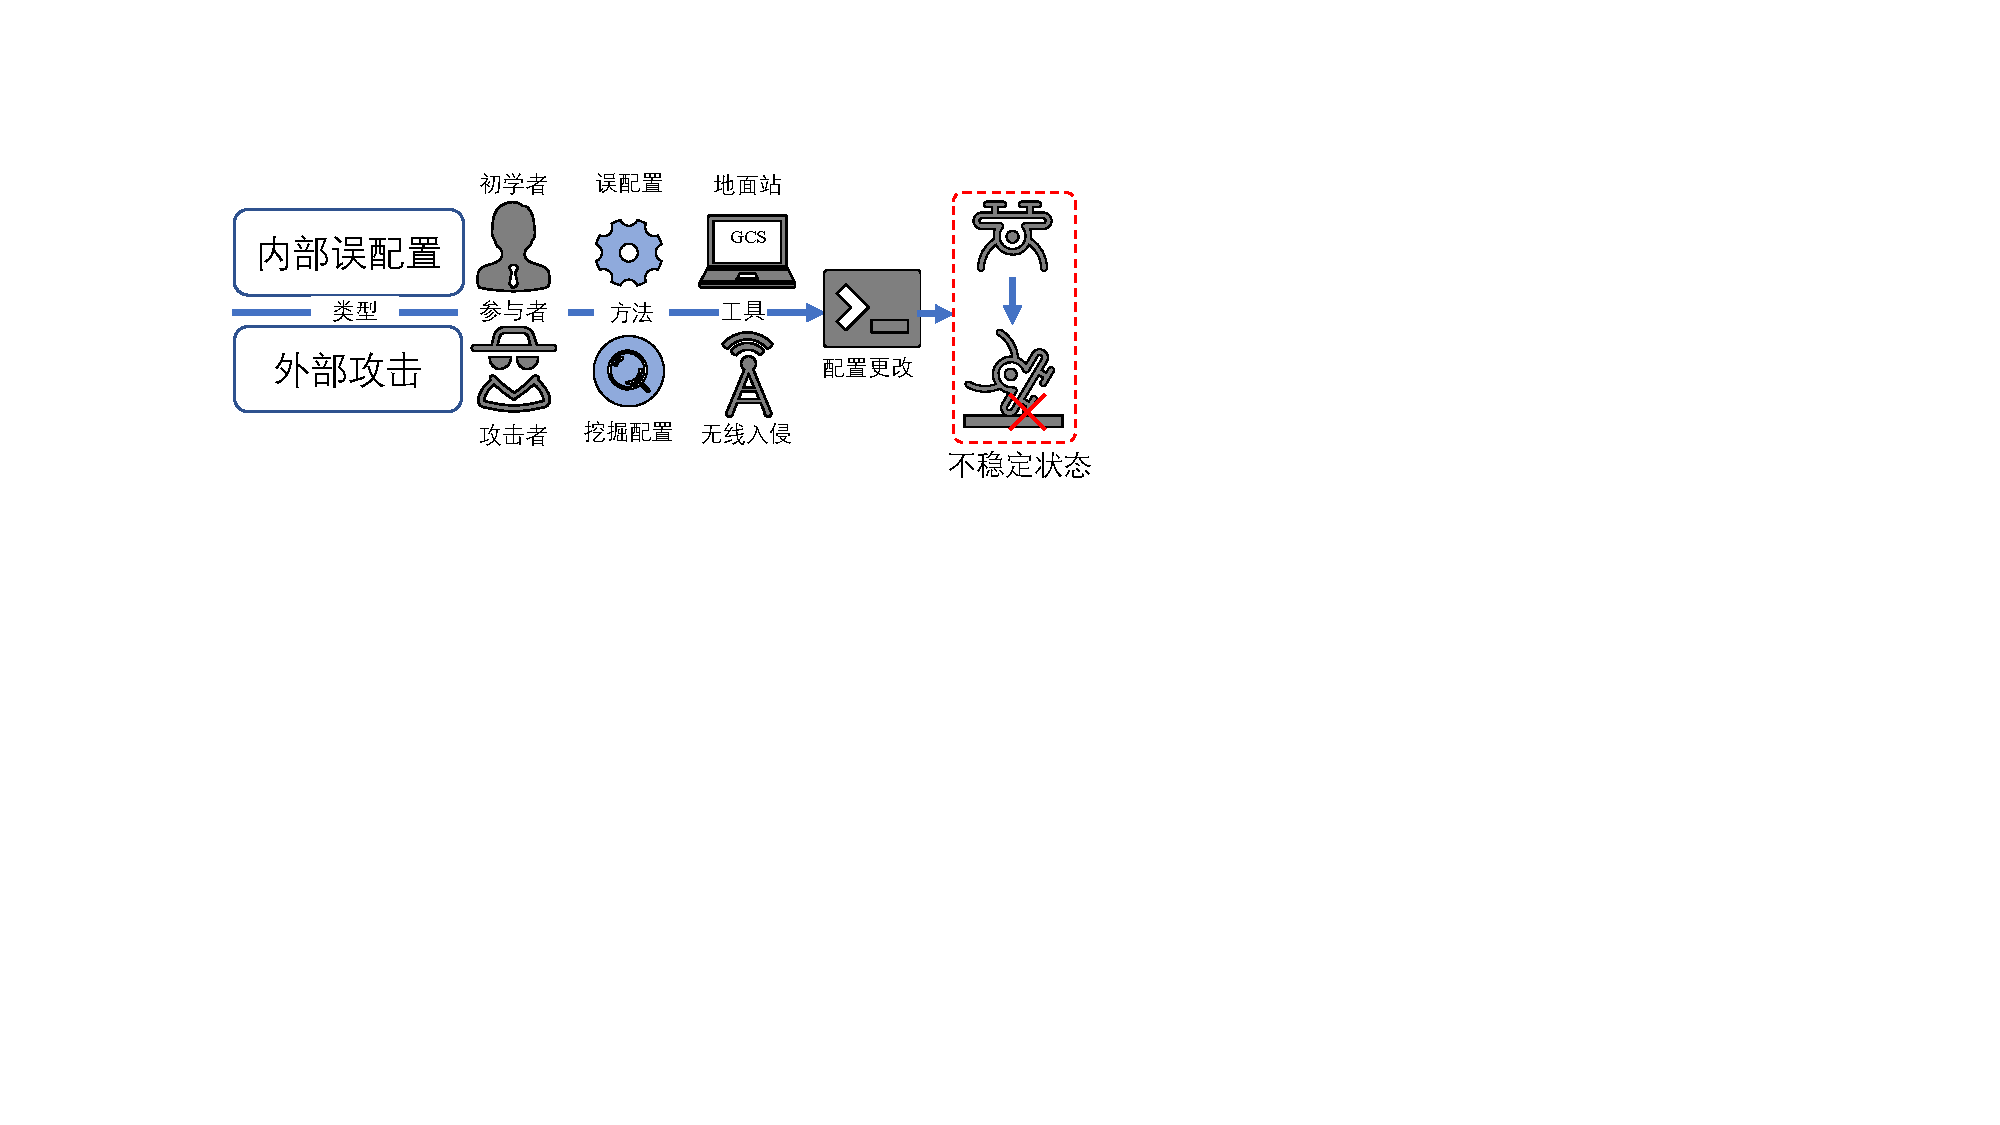
\includegraphics[width=0.9\columnwidth]{fig/background/attack.pdf}
\caption{两种情景下的威胁模型}
\label{fig:range_attack}  
\end{figure}


通常情况下,不正确的配置会导致无人机出现各种物理或系统问题。
通过飞行过程中的表现,\textit{范围实现错误}中的不正确的配置的影响可以归为以下几种情况:
\begin{enumerate}
    \item \textbf{飞行冻结:} 除非无人机正在执行降落或者悬停动作,一个正常的无人机飞行过程应该时刻保持着移动。
    然而,\textit{范围实现错误}中所出现的不正确配置可能会导致无人机在前进/后退时意外地冻结在一个航点上,或者在最小移动范围内的某个位置徘徊。
    
    \item \textbf{轨迹偏航:} \textit{范围实现错误}中的不正确的配置可能会影响无人机的飞行操控,引发重大的位置偏差。  
    这种偏差可能会导致错误的轨迹,无人机无法从中返回到正确的轨迹。
    
    \item \textbf{飞行坠毁:} 对于较小的飞行偏差,即使不是在预期的位置,无人机仍然可以安全降落。
    更糟糕的情况是,偏离导致无人机撞上一个物体,最终坠毁。

    \item \textbf{潜在动力损失:} 控制程序发送电机动力信号,驱动无人机飞行。通过调整转速从而调整其飞行姿态。
    然而,无人机电机所能做的调整是有限的。
    如果设置了\textit{范围实现错误}中的不正确配置,即使当前的油门已经使电机转速饱和到100\%,无人机控制算法仍然计算出需要更多的转速来保持飞行平衡。
    无人机持续保持这种需求状态会导致无人机飞行高度下降,甚至坠毁。

    \item \textbf{启动后的特权升级:} 在起飞前,飞行控制程序会验证配置以确定其在控制算法中的合理性。
    当发现一个或多个不正确的配置参数时,控制程序会显示一个警告信息并中止起飞操作。
    然而,如果这些被标记为不正确的配置是在起飞后被设置的,则仍然可以被飞行控制程序所接受,从而造成一系列的偏航,动力损失等后果。
\end{enumerate}

\section{挑战与解决思路}

\subsection{问题难点及挑战}
为了验证所有的配置和检测范围规范的错误,必须解决以下挑战。

\begin{itemize}
    \item \textbf{挑战 1: 如何有效地验证配置?}
先前所提出的分析飞行控制程序的方法一般是基于静态程序分析技术,他们主要搜索控制和数据的依赖关系~\cite{mayday,Believing,zhu2019new}。
然而,这种技术并不适合验证配置,因为需要分析大量的指定参数值。
传统静态分析方法只关心片段的代码,而无人机的这种配置问题需要分析整个飞行控制程序。
因为不同的参数值往往会导致涉及控制程序非常不同部分的执行流程,为了达到高代码覆盖率,若采用静态分析方法,只能对整个系统代码进行分析。
但是飞行控制程序具有巨大的代码规模(超过70万行的代码)和复杂的控制和数据依赖关系。
因此,为配置验证设计的方法必须是有效的,能够提供较高的测试覆盖率。

    \item \textbf{挑战 2: 如何高效地验证配置?}
一个配置的验证方式需要通过现实的或模拟的飞行执行进行测试。
但是由于控制参数的数量很多,每个参数的取值范围也很大。
改变参数值来生成配置并验证所有这些配置的效率很低。
维度爆炸和参数之间复杂的关联性进一步加剧了覆盖所有可能的参数组合的难度。
完成整个验证程序需要花费多至数十个小时。
因此,使用现有的方法~\cite{tartler,halin2019test}分析所有可能的配置并不适合。
另一种方法是使用模糊处理~\cite{rvfuzzer}结合二进制搜索~\cite{knuth1971optimum}来减少要分析的组合的搜索空间。
然而,该方法虽然尝试缩小搜索范围,但是由于算法本身设计的问题,无法进行多线程验证。
因此每个模糊分析迭代都需要等待,直到获得前一个配置的验证反馈。这大大增加了搜索的时间成本。


    \item \textbf{挑战 3: 如何平衡无人机的适应性和飞行稳定性的要求?}
飞行控制程序提供了广大范围的可配置参数以适应不同的飞行任务。
为了保证范围规范能够提供较大的可调整参数以保证较高的适应性,每个控制参数必须有一个大的数值范围以适应不同的情况。
同时,当其中存在的不正确配置越多,越会影响飞行稳定性。
另一方面,当参数的取值范围较小时,给参数可选择的配置是有限的,这会降低适应性,减少用户可选择的空间。
因此,复杂的飞行任务就不能进行了。
由于范围适应性和飞行稳定性的这种冲突,总结出合适的范围来平衡范围适应性和飞行稳定性是很困难的。
\end{itemize}




\subsection{解决思路}
\icsearcher 提出了以下解决方案来克服上述挑战。

\begin{itemize}

\item \textbf{解决方案1:基于灰盒的模糊测试。}
由于飞行控制程序的依赖性很复杂,简单的静态程序分析技术很难彻底的结局上述问题。
\icsearcher 的解决方法是通过灰盒的模糊分析来验证在各个配置情况下的飞行状态。
\icsearcher 采用基于GA模糊测试的方法,通过突变和验证来搜索那些高概率会影响飞行状态的配置。
该模糊测试会对配置进行突变测试,并根据反馈结果跟新下一轮需要验证的配置,配置搜索的过程是反复执行的。
这种方法解决了挑战1和2。

\item \textbf{解决方案2:飞行状态预测。}
虽然应用GA的这种模糊处理可以通过反馈机制加速参数值的搜索过程,但是仍然是一个庞大的数量。
如果使用现实/模拟执行来作为反馈机制去验证配置是非常低效的。
\icsearcher 设计了一套概率预测机制,其利用机器学习算法来训练一个状态预测器。
并使用该状态预测器的输出值来作为模糊测试中适应度评价的参考。
状态预测器不需要通过现实/模拟执行来验证配置,而是将每个配置作为输入,预测该输入会如何影响无人机的飞行状态从而来引导下一步的突变方向。
这种方法需要的时间比现实/模拟执行要少得多,以为数据标记和预测器的生成是一次性的成本。
这个解决方案解决了挑战2。

\item \textbf{解决方案3: 多目标优化器。}
为了平衡适应性和稳定性,\icsearcher 利用了一种多目标的优化方法。
该优化的方法根据检测到的不正确的配置来估计多个可行的范围指南。
优化的目标是消除不正确的配置(提高稳定性),同时为参数提供一个更宽的范围(提高适应性)。
多目标优化的每个解决方案(即范围指南)都是特定条件下的最佳解决方案,即适应性和稳定性的最佳平衡。
这种多目标优化结果方法允许用户根据他们的要求从多个范围指南中选择一个合适的范围。
这种方法解决了挑战3。
\end{itemize}


\section{方案}
为了有效且高效地查找出\textit{范围实现错误}所带来的那些不正确配置,本章节详细的介绍一种新的轻量化搜索工具\icsearcher ,其利用GA来进行突变模糊搜索来发现潜在的不正确配置。

\subsection{概览}

\begin{figure}[ht]
  \centering
    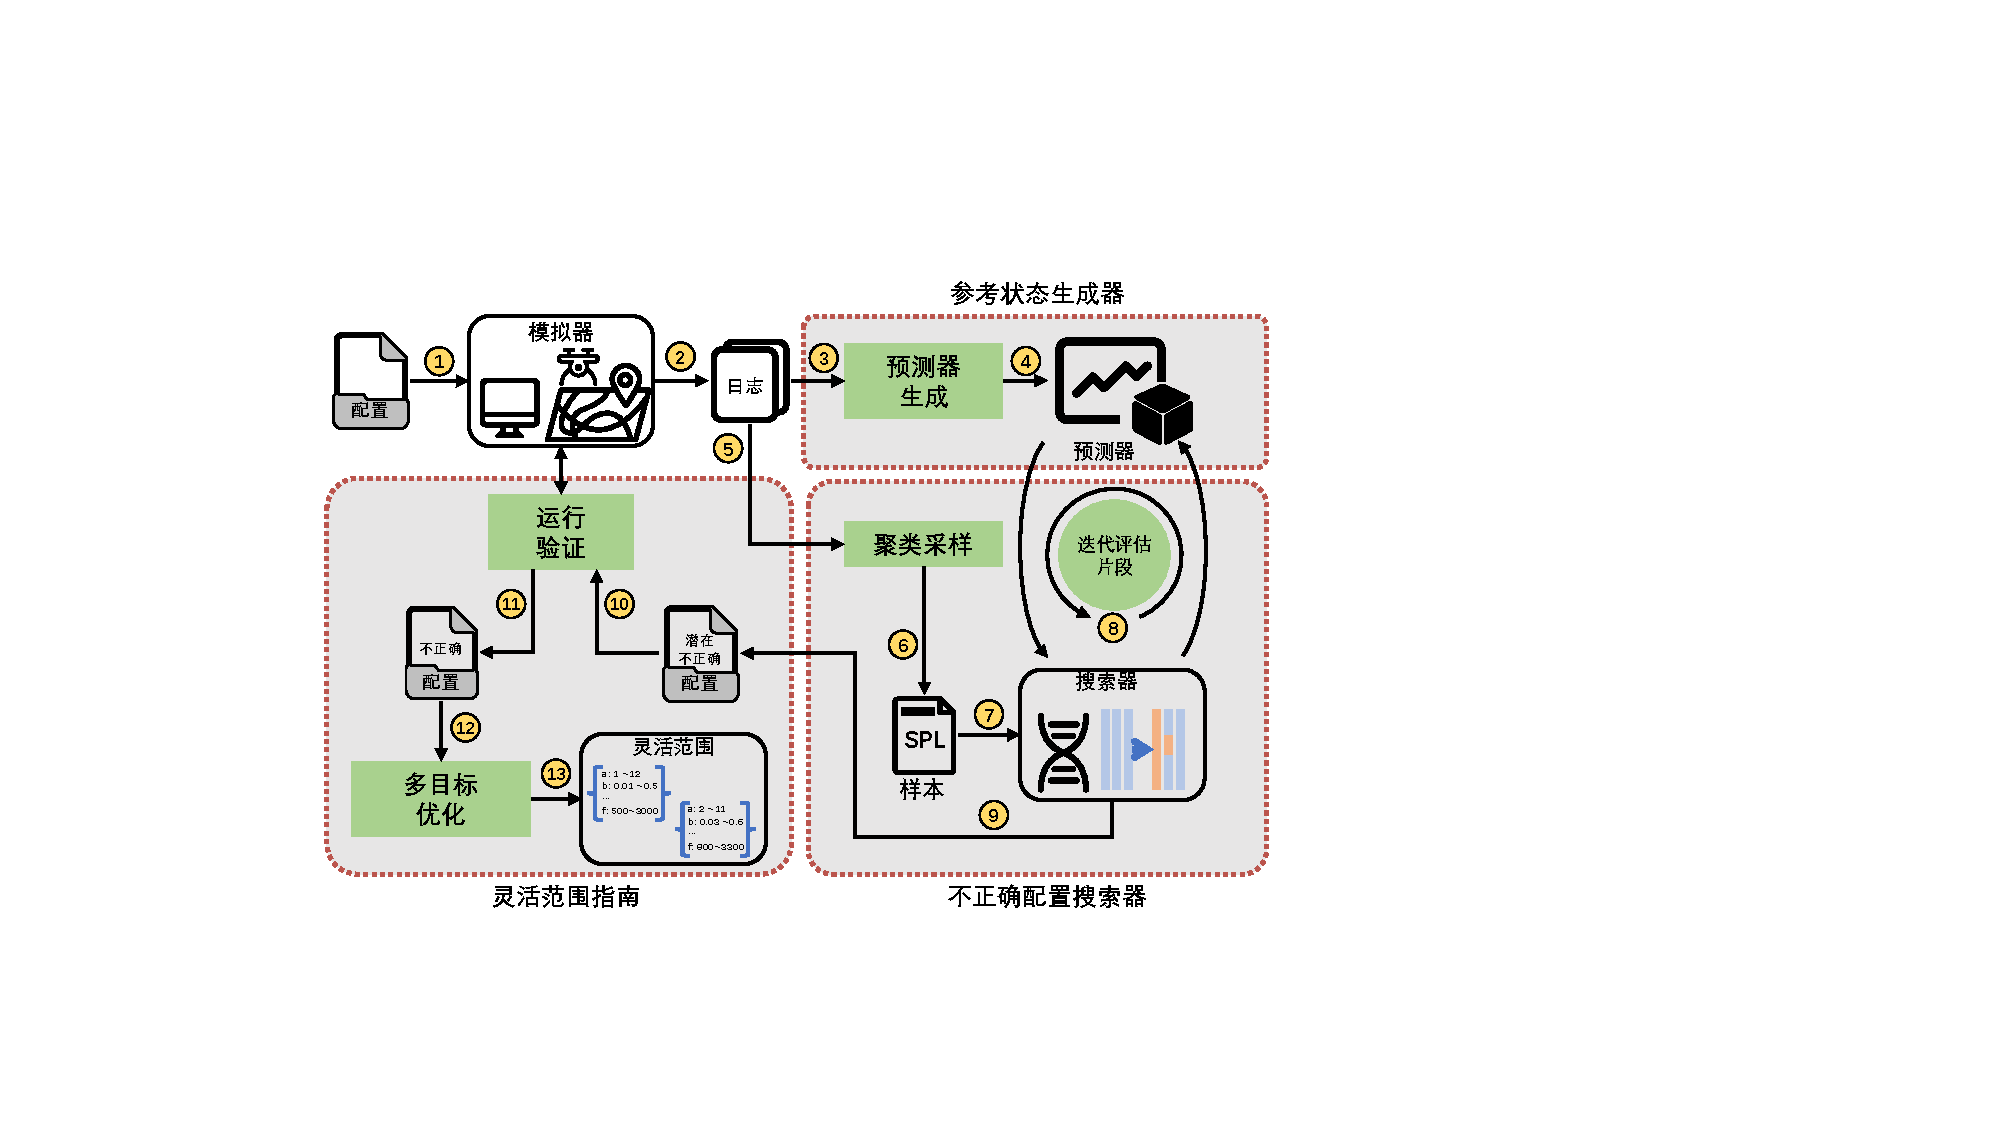
\includegraphics[width=\columnwidth]{fig/range/range_overview.pdf}
\caption{\icsearcher 流程概览.}
\label{fig:range_overview} 
\end{figure}

图~\ref{fig:range_overview}展示了\icsearcher 的整体框架所包含三个部分,包括\emph{参考状态生成器}、\emph{不正确配置搜索器}、和\emph{灵活范围指南},其各自功能的简单描述如下:

\begin{itemize}
\item \textbf{参考状态生成器:} 它采用历史飞行数据并创建一个预测器来预测飞行的状态变化,后续模块利用它来评估不正确的配置。
\item \textbf{不正确配置搜索器:} 它使用GA搜索模块来产生潜在的不正确配置。

\item \textbf{灵活范围指南:} 它应用多目标优化来提供安全的范围指南。

\end{itemize}

\icsearcher 的整体工作流程如下描述。
首先,由于预测器的生成和搜索器的搜索过程需要各种飞行数据。
\icsearcher 会利用一个模拟器并通过反复执行无人机飞行任务从而产生大量在不同的配置下的飞行数据(\circled{1}\circled{2})。
飞行日志数据被分成两部分,一部分被参考状态预测器采用用来生成预测器(\circled{3}),另一部分为搜索器提供关于飞行状态和传感器数据的基础数据(\circled{5})。
通过这些日志数据,系统训练一个能预测状态根据配置变化的预测器(\circled{4})。
对于不正确的配置搜索器,它对首先数据进行聚类,并从每个聚类组中抽取代表样本(\circled{6}\circled{7})。
然后搜索器会进一步针对这些样本进行启发式搜索,发掘潜在的不正确配置(\circled{8})。
比较特殊的是,在该搜索过程中,系统迭代地使用预测器来评估哪种配置有更高的概率导致不稳定状态。
搜索器的启发式搜索将在特定条件得到满足时停止。
当每个样本都通过搜索器获得了相应的潜在不正确配置后,他们会被构建成一个集合(\circled{9}),并通过模拟器飞行任务执行进行验证(\circled{10}\circled{11})。
最后,根据潜在不正确配置的验证结果,灵活的范围指南利用多目标优化来完善多个可用的可行范围指南,这些指南在某些特定条件下满足可用性和稳定性的最佳平衡(\circled{12}\circled{13})。

\subsection{飞行数据收集}\label{subsec:log_gen}
参考状态预测器是一个拥有未知参数的灰盒模型,需要大量数据进行拟合。
由于没有描述无人机输入/输出的标准数据集,为了构建一个预测器并为进一步搜索提供状态样本,该方案建立了一个飞行测试场景来收集飞行日志。
由于非默认配置的飞行可能导致不稳定的飞行,并进一步造成硬件损坏,对于飞行测试场景,该方案利用模拟飞行来收集飞行日志。
值得注意的是,考虑到强逆风或顺风等环境因素,即使使用默认配置,仍然可能发生崩溃。
这些飞行测试设定了不同的配置但设置了相同的飞行任务\tool{AVC2013}~\footnote{\url{https://avc.sparkfun.com/2013}},该任务通常用于测试无人机任务执行能力的,
对于用于训练预测器的数据,系统记录了飞行日志但舍弃了那些造成不稳定状态的,因为它们是不可控的和复杂的(与稳定状态数据相比)。
无人机中的不同数据模块有不同的类型的日志记录频率,本方案将其统一为10Hz,即0.1秒的间隔。
每个日志条目包含的状态信息包括角位置、角加速度、油门速度、GPS、陀螺仪和加速度计的传感器数据、当前设定的配置和时间戳索引。
对于该方案讨论的飞行控制程序,\tool{Ardupilot}和\tool{PX4},实验为 \tool{Ardupilot}记录了$740,799$的系统日志条目,为 \tool{PX4}记录了$410,962$的系统日志。
    
\subsection{参考状态预测器}
虽然利用GA模糊法可以减少参数的搜索空间,但参数组合(配置)的数量仍然很多,这使得通过现实/模拟执行进行验证的效率很低。
规避了采用飞行执行验证方式,本方案利用预测器来验证配置的影响对于无人机飞行的影响。
根据背景介绍中的说明,飞行控制算法根据之前的状态反馈、当前状态、传感器数据和加载的配置来估计下一个参考状态。
本方案应用机器学习(Machine Learning)预测器来模仿这个过程,学习他们的输入/输出相关性。
与原来的控制算法不同,由于预测器是用来拟合控制算法的,为了提高准确性,本方案的预测器考虑了多个历史反馈状态数据作为输入。
使用这种方法生成的预测器具有与控制算法相同的属性,可以估计参考状态,并且后续可以进一步评估配置如何影响飞行状态。
训练预测器的生成主要通过\emph{特征提取}和\emph{预测器生成}两个步骤所完成。


\subsubsection{特征提取}
无人机的日志条目中包含了许多无关信息,\icsearcher 通过选择特定的数据来构建特征向量。
因为并非条目中的所有项目在不稳定场景的影响下都具有可变偏差。
例如,即使无人机的姿态受到干扰,位置状态(高度、纬度、经度)也不会发生剧烈变化。
同样,温度传感器数据在整个任务过程中基本保持不变。
\param{BATT2\_VLT\_OFFSET}(电压偏移调整)和 \param{COMPASS\_OFS\_X}(X 轴上的罗盘偏移,单位为毫高斯)等参数不会影响姿态。
由于该方案的目标是分析影响飞行姿态(即角度和速度)的不稳定状态,因此在选取特征时主要考虑以下状态、传感器数据和配置。
(1) 飞行状态的角度位置和速度,表示为$a$。
(2) 从陀螺仪、加速度计和罗盘获得的传感器数据,表示为$e$。
(3) 调节姿态的控制或任务的参数集,表示为$c$。
根据上述信息,系统将它们分组为一个特征向量,$v\{a, e, c\}$,为了便于描述,定义$s=\{a,e\}$。
因此,在时间戳$t$时的数据所组成的特征向量应该为$v_t=\{s_t,c_t\}$。
这些向量被进一步组合以构建一个特征矩阵。

\subsubsection{预测器生成}
由于长短时记忆网络(LSTM)~\cite{hochreiter1997long}技术能有效地拟合复杂的输入/输出关系~\cite{stock,highway,selvin2017stock},\icsearcher 使用\tool{LSTM}作为预测器来预测下一个参考状态。
预测器将时间戳小于等于$t$的若干$h$连续向量作为输入(即$V\{v_{t-h-1},...,v_{t-1},v_{t}\}$),从而预测输出下一个预测的向量$v'_{t+1}$中的参考状态$a'_{t+1}$,后续的实验将会确定使用多少个历史向量$h$较为合适。
在训练阶段,LSTM采用\tool{平均平方误差 (Mean Squared Error,MSE)}~\cite{4775883}来迭代优化预测器的内部权重,确保预测的状态$a_{t+1}'$足够接近于地面真实状态$a_{t+1}$。

虽然预测器是指定给某个控制程序的,但预测方案是可以根据相应的控制程序(即动态模型、控制算法、配置参数和数据采样方法)来扩展的。
也就是说,虽然为某一控制程序生成的预测器不能直接用于其他控制程序,但是生成预测器的模板是通用的,不同的飞行控制程序可以提取相同的格式状态和传感器数据来实例化预测器以估计参考状态。

\subsection{不正确配置搜索器}
为了搜索引发不稳定偏差(即参考状态和当前状态之间存在严重偏差)的不正确配置,本搜索方案以历史飞行数据中存在的飞行状态为基础,开展模糊搜索测试以找出具有高概率导致这个基础状态出现较高偏差的潜在配置。
方案从历史的飞行数据中聚类出具有代表性的状态片段样本,然后从用遗传算法(GA),一种元启发式搜索的方法搜索在该状态样本的背景下,什么样的配置会引发参考状态和实际状态出现偏差变大的情况(即产生不稳定), 并将这些配置称之为\emph{潜在不正确配置}。

具体而言,对于排除了配置元素的$N$个原始飞行条目$Raw=\{v_{1},v_{2},...v_{N}\}$,搜索器首先将其分成多个段$S_{t}, t \in [1,N]$ 作为候选片段。
具体的每个段得生成方式如下。
\begin{equation}
    S_{t}=\{v_{t},v_{t+1},...,v_{t+len-1}\}, t~mod~(t+len) = 0
\end{equation}
其中$t$是记录数据的索引,$len$是每个片段的长度。
飞行过程中的噪声或者瞬时误差都会对预测器产生影响,因此,为了排除瞬时误差对整个搜索的影响,搜索器将每个段的长度设定为$10+h$(即$len=10+h$)。
同时由于重复配置的相似段数据可能会降低搜索效率,因此,系统采用先聚类后抽样的方法选择有代表性的样本进行搜索,这样可以在保持多样性的同时减少冗余。
\icsearcher 首先使用\tool{DBSCAN}~\cite{schubert2017dbscan},一种基于概率密度的非参数自适应聚类算法,对这些样本数据片段进行聚类,并从每个聚类组中随机抽取$m_{2}$个代表数据样本。
对于每一个数据片段,GA搜索器启动,依靠突变、交叉和选择这些遗传算法的迭代流程来进行搜素相应的不正确配置。
最后,所有样本片段的搜索结果都被合并且去掉重复,成为一个独特的集合,被称为\emph{潜在不正确配置集合}。
接下来的内容将详细介绍关键的步骤,即关于如何评估配置的 \emph{预测器片段评估}和关于搜索器如何工作的\emph{搜索过程}。

\subsubsection{预测器片段评估}
通过使用预测器,GA搜索应用适应度来量化一个配置在特定环境(状态和传感器数据)下可能造成的偏差程度。
预测器对于片段数据的评估创建了一个得分来描述该配置可能造成的偏差的。
分数越高,说明预测器认为这种配置越是\dquote{危险},否则就越是\dquote{安全}。

假设当前的模糊搜索是针对上下文片段$S\{v_{1},v_{2},...,v_{10+h}\}$进行的。
给定一个待评估的配置$c\{p_1,p_2,...,p_{n2}\}$($n2$是参数的数量)时。
片段评估函数将其与段合并以创建特征向量$V\{\{v_1, c\}, \{v_2, c\},...,\{v_{10+h}, c\}\}$。
然后,该函数用一个滑动窗口将$V$分成长度为$h+1$的块。
\begin{equation}
    B = \{b_{1}, b_{2}, ..., b_{10}\} 
\end{equation}  
其中每个块$b_{t}$ 是:
\begin{equation}
    b_{t} = \{v_{t}, v_{t+1}, ..., v_{t+h}\}, t\in[1, 10] 
\end{equation}
对于每个块$b_{t}$,$b_{in}=\{v_t,v_{t+1},...,v_{t+h-1}\}$被用作输入,$v_{t+h}$中的$a_{t+h}$被用作真实状态数据。
也就是说$b_{in}$被作为预测器的输入用来估计参考状态$a'(t+h)$。
一个单一的偏差是预测状态和真实状态之间的一范数,也就是$d = \Vert a_{t+h} - a'_{t+h} \Vert$。  
而一个片段包含有$10$个块,也就可以划分$10$组输入和真实输出。
进一步的也就能够计算出10个偏差$D=\{d_1, d_2, ..., d_{10}\}$,对应到原始数据当中,也就是$1$秒内的偏差。
这个配置$c$的适应度评价是这些偏差的总和$D_{sum}=\sum_{i=1}^{10}{d_i}$。
搜索的目标是找出那些被预测为适配度最大化的配置,也就是有较大概率引起不稳定状态的个体(此处指配置)。


\subsubsection{搜索流程}
对于一个片段数据$S$,搜索器分配具有默认参数值的种群(配置组),种群中的每一个个体表示一个配置。
假设种群大小为$NP$,最大迭代次数为$G_{max}$。
搜索过程中对该种群进行反复变异和更新,具体过程如下。

假设当前迭代代数为第$g$代($g\in[1,G_{max}]$),搜索器首先对当前种群
\begin{equation}
pop_g=\{c_{1,g},c_{2,g}...,c_{NP,g}\}   
\end{equation}
进行变异,生成变异种群
\begin{equation}
pop_v=\{y_{1,g},y_{2,g},...,y_{NP,g}\}
\end{equation}
变异种群的每个配置都是按以下方式计算。
\begin{equation}
    y_{i,g} = c_{i,g} + F * (c_{best,g} - c_{i,g}) + F * (c_{r1,g} - c_{r2,g})
\end{equation}
其中$c_{r1/r2,g}$为种群中的一个随机个体(配置)。
$c_{best,g}$是那一代中最佳适应度的个体,而$F$为比例因子。

然后搜索器对$pop_g$和$pop_v$进行交叉运算,产生一个新的实验种群:
\begin{equation}
    pop_e=\{ec_{1,g},...,ec_{NP,g}\}
\end{equation}
其中
\begin{equation}
    ec_{i,g}=\{ec_{i1,g},ec_{i2,g},...,ec_{ij,g}\},i \in [1,NP], j \in[1,D]
\end{equation}
一个配置中的参数值$ec_{ij,g}$可按如下方式获得:
\begin{equation}
    ec_{ij,g}=\begin{cases}
y_{ij,g}, & if~rand(0,1) < CR~or~j=j_{rand}\\
c_{ij,g}, & otherwise
\end{cases}
\end{equation}  
其中$j_{rand}$是$[1,D]$中的一个随机整数、
$CR$是交叉率、
$c_{ij,g}$是$pop_g$中第$i$配置的第$j$个参数值、
和$y_{ij,g}$是$pop_v$中第$i$种配置的第$j$个参数值。

搜索器使用\emph{预测器片段评估}中的方法来计算$pop_g$和$pop_e$中个体的分数。
根据它们的得分,搜索者从群体中选择配置,用以下方法创建下一代$pop_{g+1}$:
 \begin{equation}
    c_{i,g+1}=\begin{cases} 
ec_{i,g}, & if~f(ec_{i,g})<f(c_{i,g})\\
c_{i,g}, & otherwise
\end{cases}
\end{equation}   
其中$f$是\emph{预测器片段评估}。

最终,如果种群的适应性不再增加,或者迭代达到最大数量$G_{max}$。
搜索器就会停止,最后一代种群中得分最高的前$10$的个体被认为是潜在的不正确配置。
    
\subsection{灵活范围指南}
根据搜素器提供的潜在不正确配置,\icsearcher 需要总结出一个新的范围指南。
使用者在参考这个范围指南后会减少出现不正确配置的可能性,从而进一步减少触发不稳定飞行状态的可能性。

\subsubsection{执行验证} 
搜索结果是潜在不正确的配置,意味着这些配置有很高的概率导致不稳定的状态,但是它们是否是不正确的仍然需要通过飞行执行测试来验证。
因此,\icsearcher 利用飞行模拟器平台来测试这些配置对无人机飞行带来的影响,观察哪些配置会导致真正的不稳定状态。
与收集阶段类似,无人机用这些配置设置来执行\tool{AVC2013}任务。

\subsubsection{范围指南生成} 
参数范围指南的目标是防止用户上传不稳定的配置。
但是上述搜索器所发现的不正确配置是离散地存在于可配置空间中的,而范围指南只能是连续的可配置空间,因此就面临一个问题。
给出较小的可配置空间确实能够极大地避免不正确配置地空间,有效地确保了稳定性。
但是相应地,其可配置的范围变小,这并不利于用户的实际使用需求,也就是降低了适应性。
因此,\icsearcher 不提供一个具体的范围指南,而是利用多元优化来确定灵活的范围指南。
\icsearcher 主要基于以下考虑提供灵活的范围指南。
(1)随着参数数量的增加,很难完全排除不安全的参数值,因为安全参数范围可能不连续。
(2)虽然稳定性是最重要的,用户可能愿意为更好的控制灵活性或可用性承担一些小的风险。
如果一个配置中的所有参数值都在指南规定的范围内,则认为该配置已被覆盖。
\icsearcher 将范围指南($Range'$)的生成视为以下优化问题。

\begin{equation}
\begin{cases}
        min~f_1 = \frac{num(R_{incorrect } \in Range')}{num(R \in Range')}   \\
       max~f_2 = num(R \in Range')  \\
       s.t. &\\
       Range' \in OriginRange
\end{cases}
\label{eq1}
\end{equation} 

优化问题涉及两个目标:
(1) 尽可能利用验证结果,使指南所涵盖的验证配置$R$的数量最大化。
(2)尽可能保持安全,以最小化不正确配置的覆盖范围$R_{incorrect}$。
实际上,缩小不正确配置的覆盖范围也会缩小每个参数值的范围,反之亦然。
因此,与其为每个参数定义严格的范围。
系统用多个约束条件来解决这个优化问题,以构建一个多样化的\tool{Pareto}边界解决方案组。
这些\tool{Pareto}解决方案形成了一个由最佳可行方案组成的边界。
允许用户可以从边界位置选择最符合他们需的方案来平衡他们任务的要求中的安全性和适应性。 



\section{实验结果及分析}
本章节通过考虑其在验证配置方面的有效性和效率来评估\icsearcher 。
\begin{itemize}
 
\item \textbf{研究问题1 有效性:} \icsearcher 能精确检测出来少不正确的配置?

\item \textbf{研究问题2 适应性:} \icsearcher 可以为参数提供最合适的值范围?

\item \textbf{研究问题3 提升:} 突变和预测器是如何帮助改善配置验证的?

\end{itemize}

\subsection{实验设定}

\begin{itemize}
    \item \textbf{实验程序:}
本章节将 \icsearcher 应用于两个流行的开源飞行控制程序。
\tool{ArduPilot} (4.2.0)~\cite{ardupilot} 和 \tool{PX4} (1.13)~\cite{px4}, 这些工具被无人机制造商广泛使用,如\tool{Parrot}、\tool{Mamba}和\tool{Mateksys}~\footnote{\url{https://ardupilot.org/copter/docs/common-autopilots.html\#closed-hardware}}。

\item \textbf{测试设备:}
为了验证\tool{ArduPilot}和\tool{PX4}中规定的配置,本此实验利用四个实验飞行器(如图~\ref{fig:range_pix}所示)进行测试,其中包括两个装有\tool{Pixhawk}的无人机~\cite{meier2011pixhawk}。(\tool{CUAV ZD550}和\tool{AMOVLab Z410}),两个无人机模拟器(\tool{Airsim}~\cite{airsim2017fsr},\tool{Jmavsim}~\footnote{\url{https://dev.px4.io/v1.10_noredirect/en/simulation/jmavsim.html}})。

\begin{figure}[htb]
\centering{
\subfloat[CUAV ZD550]{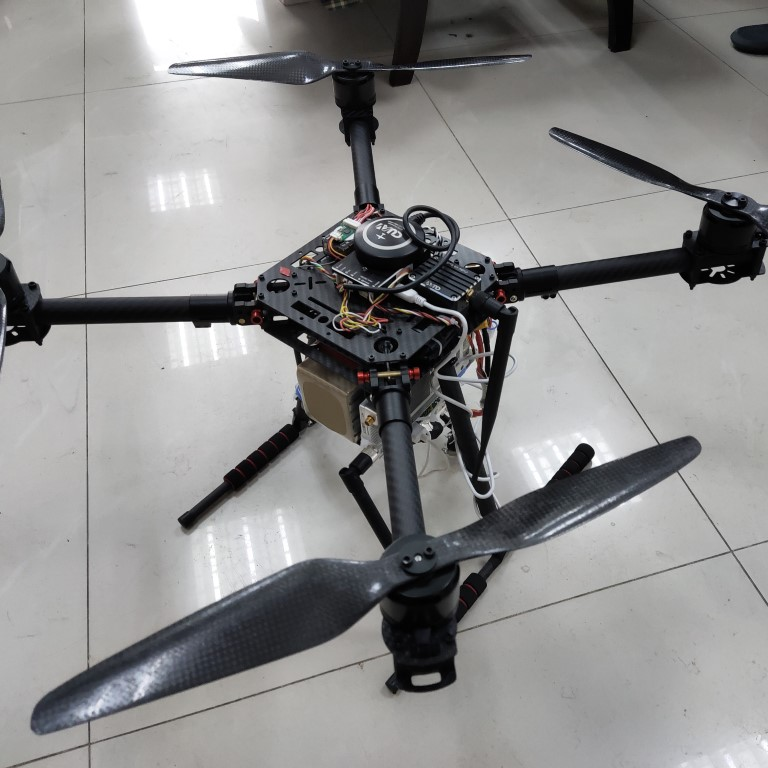
\includegraphics[width=0.3\linewidth]{fig/range/real/px1.jpg}}\quad
\subfloat[AMOVLab Z410]{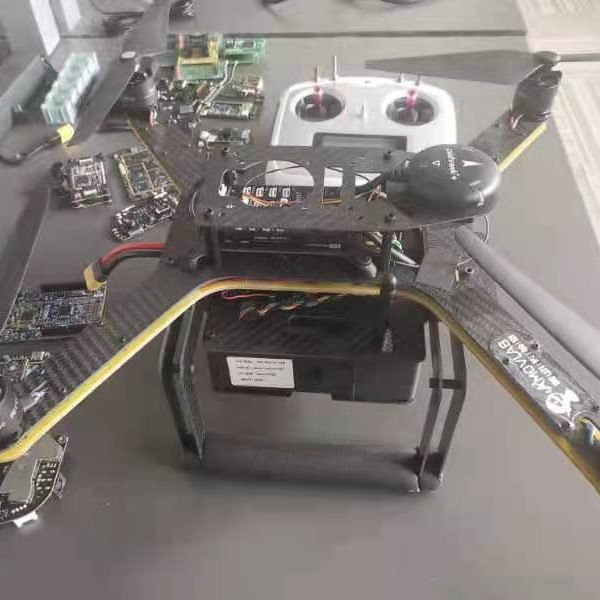
\includegraphics[width=0.3\linewidth]{fig/range/real/px2.jpg}}
}

\centering{
\subfloat[Airsim]{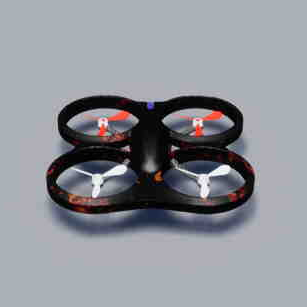
\includegraphics[width=0.3\linewidth]{fig/range/real/airsim.png}}\quad
\subfloat[Jmavsim]{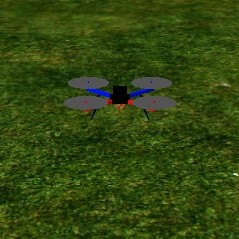
\includegraphics[width=0.3\linewidth]{fig/range/real/jmavsim.jpg}}}
\caption{用于实验的真实和虚拟无人机车辆}
\label{fig:range_pix}
\end{figure}

\item \textbf{参数选择:}
根据制造商提供的控制参数描述。
后续实验为\tool{Ardupilot}选择了20个参数(表~\ref{tab:range_paramall}),为\tool{PX4}选择了14个参数(表~\ref{tab:range_paramall_px4}),可能影响飞行角位置和角速度。
需要说明的是,一个预测器对特定的飞行控制程序是有效的,所以对于\tool{Ardupilot}和\tool{PX4}使用相同的架构结合各自的数据分别产生预测器。


\begin{table*}[htb]
\centering
\begin{minipage}{0.49\linewidth}
\small
\caption{用于实验的Ardupilot控制程序的参数}
\label{tab:range_paramall}
\centering
\begin{tabular}{ccc}
        \toprule[1.5pt]
         参数 & 官方范围 & 默认值 \\
        \midrule[0.8pt]
         PSC\_VELXY\_P & [0.10, 6.00] & 2.0 \\ 
       
         PSC\_VELXY\_I & [0.02, 1.00] & 1.0 \\
       
         PSC\_VELXY\_D & [0.00, 1.00] & 0.5 \\
       
         PSC\_ACCZ\_P & [0.20, 1.50] & 0.5 \\
       
         PSC\_ACCZ\_I & [0.00, 3.00] & 1.0 \\
       
         ATC\_ANG\_RLL\_P & [3.00, 12.0] & 4.5 \\
       
         ATC\_RAT\_RLL\_P &  [0.01, 0.50] & 0.135 \\
        
         ATC\_RAT\_PIT\_I & [0.01, 2.00] & 0.135 \\
        
         ATC\_RAT\_RLL\_D & [0.00, 0.05] & 0.0036 \\
        
         ATC\_ANG\_PIT\_P & [0.00, 12.0] & 4.5 \\
       
         ATC\_RAT\_PIT\_P & [0.01, 0.50] & 0.135 \\
        
         ATC\_RAT\_PIT\_I & [0.01, 2.0] & 0.135 \\
        
         ATC\_RAT\_PIT\_D & [0.00, 0.05] & 0.0036 \\
       
         ATC\_ANG\_YAW\_P & [3.00, 12.0] &4.5 \\
       
         ATC\_RAT\_YAW\_P & [0.10, 2.50] & 0.18 \\
       
         ATC\_RAT\_YAW\_I & [0.01, 1.00]& 0.018 \\
       
         ATC\_RAT\_YAW\_D & [0.00, 0.02] & 0 \\
         
         WPNAV\_SPEED & [20, 2000] & 500 \\
       
          WPNAV\_ACCEL & [50, 500]& 100 \\
       
       ANGLE\_MAX & [1000, 8000] & 4500 \\
        \bottomrule[1.5pt]
\end{tabular}
\end{minipage}
\begin{minipage}{0.49\linewidth}
\small
\caption{用于实验的PX4控制程序的参数}
\label{tab:range_paramall_px4}
\centering
\begin{tabular}{ccc}
        \toprule[1.5pt]
          参数 & 官方范围 & Default \\
        \midrule[0.8pt]
         MC\_ROLL\_P & [0.00, 12.0] & 6.5 \\
       
         MC\_PITCH\_P & [0.00, 12.0] & 6.5 \\ 
       
         MC\_YAW\_P & [0.00, 5.0] & 2.8 \\ 
        
         MC\_YAW\_WEIGHT & [0.00, 1.00] & 0.4 \\ 
        
         MPC\_XY\_P & [0.00, 2.00] & 0.9 \\ 
        
         MPC\_Z\_P & [0.00, 1.50] & 1.0 \\ 
        
         MC\_PITCHRATE\_P & [0.01 0.60] & 0.15 \\ 
        
         MC\_ROLLRATE\_P & [0.01, 0.50] & 0.15  \\ 
        
         MC\_YAWRATE\_P & [0.00, 0.60] & 0.2 \\ 
        
         MPC\_TILTMAX\_AIR & [20.0, 89.0] & 45.0 \\ 
        
         MIS\_YAW\_ERR & [0.00, 90.0] & 12.0 \\
        
         MPC\_Z\_VEL\_MAX\_DN & [0.5, 4.0] & 1.0 \\
        
         MPC\_Z\_VEL\_MAX\_UP & [0.5, 8.0] & 3.0 \\
        
         MPC\_TKO\_SPEED & [1.0, 5.0] & 1.5  \\
        
        \bottomrule[1.5pt]
\end{tabular}
\end{minipage}
\end{table*}

\item \textbf{模型和搜素设定:}
预测器和GA搜索器是用Python实现的。
对于GA,其进化停滞判断阈值被设定为$0.1$、代表数$m_{2}$被设定为$10$、最大的进化代数被设定为$200$、
初始种群的大小为$500$(即$NP=500$)、比例因子$F$为0.4。

\end{itemize}


\subsection{研究问题1: 有效性}
实验首先对\icsearcher 在\tool{Ardupilot}和\tool{PX4}两个不同飞控情况下进行评估,计算了飞行状态预测阶段预测器的预测精度。
然后实验验证了预测的不正确配置是否会影响飞行稳定性。

\subsubsection{状态预测}
首先利用章节~\ref{subsec:log_gen} 中的日志数据为 \tool{Ardupilot} 和 \tool{PX4} 创建预测器,其中 90\% 的数据用于训练,10\% 用于测试。
最后根据实验结果确定最佳输入长度$h$。
预测器的预测精准度结果如表~\ref{tab:range_acc}所示。
从表中可以观察到,不同长度的输入会对预测的准确性产生轻微的影响。
为了后续实验的准确性,根据这些结果,后续实验选择精度最好的预测器,即输入长度h=4来进行相关的测试。

\begin{table}[ht]
\caption{不同输入长度的测试数据的预测精度}
\label{tab:range_acc}
\centering
\begin{threeparttable}
\begin{tabular}{c|ccccc}
        \toprule[1.5pt]
        $h$  & 2 & 3 & 4 & 5 & 6 \\
        \midrule
        

        Ardupilot  & 96.05\% & 96.19\% & 97.10\% & 95.60\% & 95.77\% \\

        PX4 & 94.32\% & 95.56\% & 96.15\%  & 94.52\% & 94.45\% \\

        \bottomrule[1.5pt]
\end{tabular}
% \begin{tablenotes}
% \footnotesize
% \item[*] Ardu is Ardupilot.
% \end{tablenotes}
\end{threeparttable}
\end{table}

此外,实验选择了两个个飞行日志(\tool{Ardupilot}和\tool{PX4})中的数据用来展示了预测和实际状态变化之间的差异。
通过将日志中的数据进行相同的预处理操作并输入到训练好的预测其中输出预测结果。
图~\ref{subfig:range_diff1} 和图~\ref{subfig:range_diff2} 中展示了预测器输出的预测状态和实际状态的的对比图。
图中虚线曲线表示实际状态,实线表示预测状态,底部的直方图(青色条)表示两条曲线之间的差异。
该图表明预测器准确地预测了状态变化的趋势,与实际值非常匹配。



\begin{figure*}[htb]
\centering
\begin{minipage}{0.49\linewidth}
    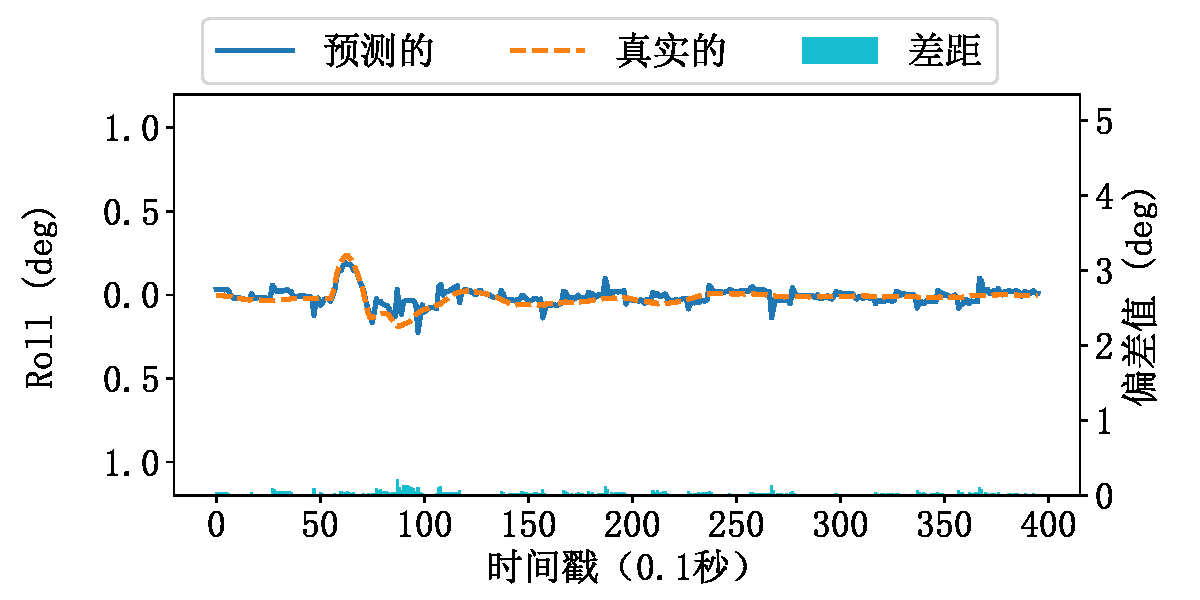
\includegraphics[width=\linewidth]{fig/range/ardu_real_roll.pdf}\quad
    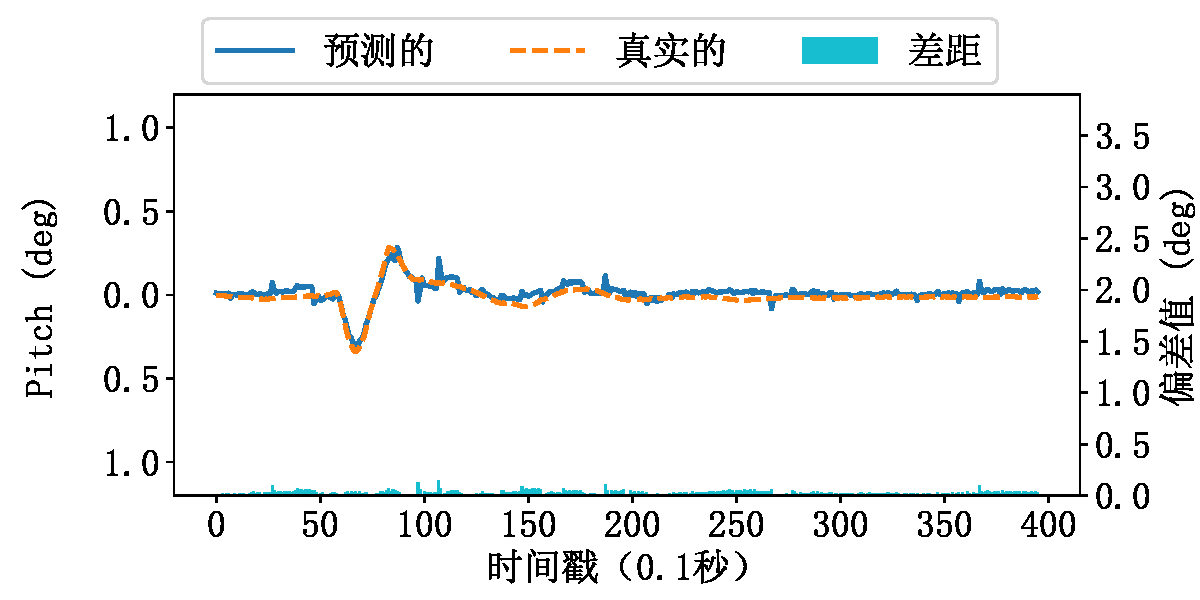
\includegraphics[width=\linewidth]{fig/range/ardu_real_pitch.pdf}\quad
    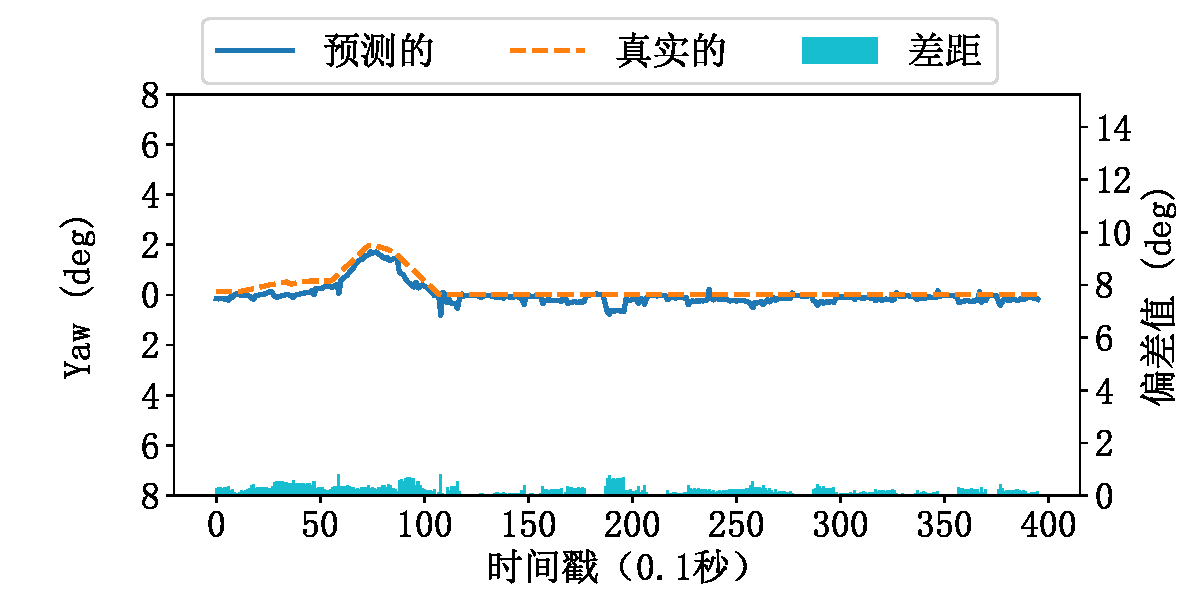
\includegraphics[width=\linewidth]{fig/range/ardu_real_yaw.pdf}
    \caption{Ardupilot 状态变化(Roll, Pitch, 和 Yaw)}
    \label{subfig:range_diff1}
\end{minipage}
\begin{minipage}{0.49\linewidth}
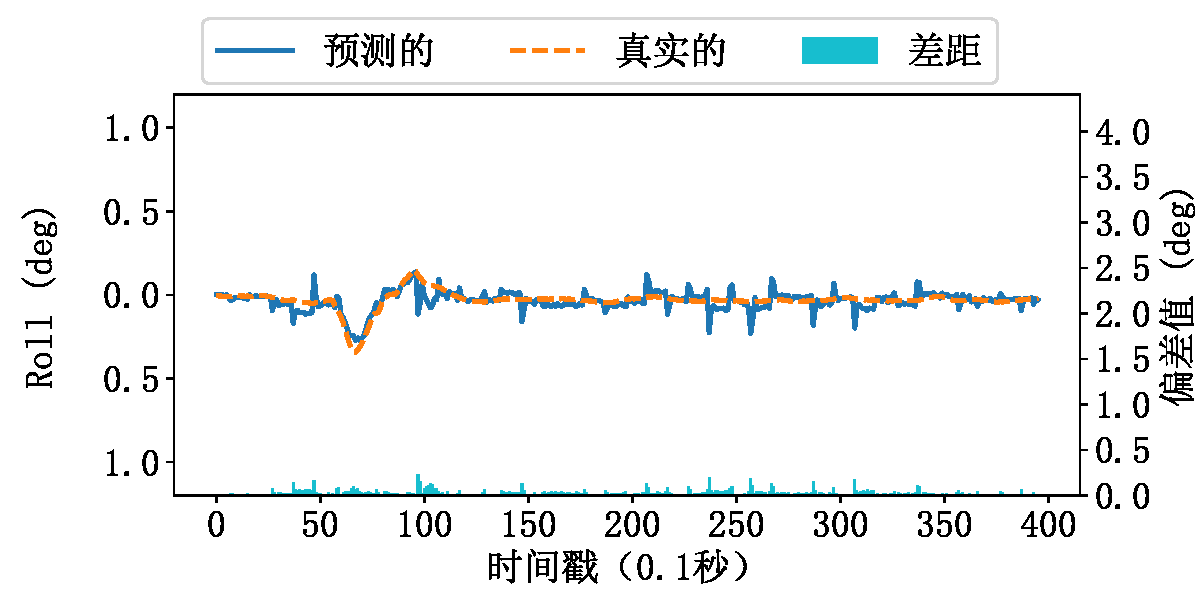
\includegraphics[width=\linewidth]{fig/range/px4_real_roll.pdf}\quad
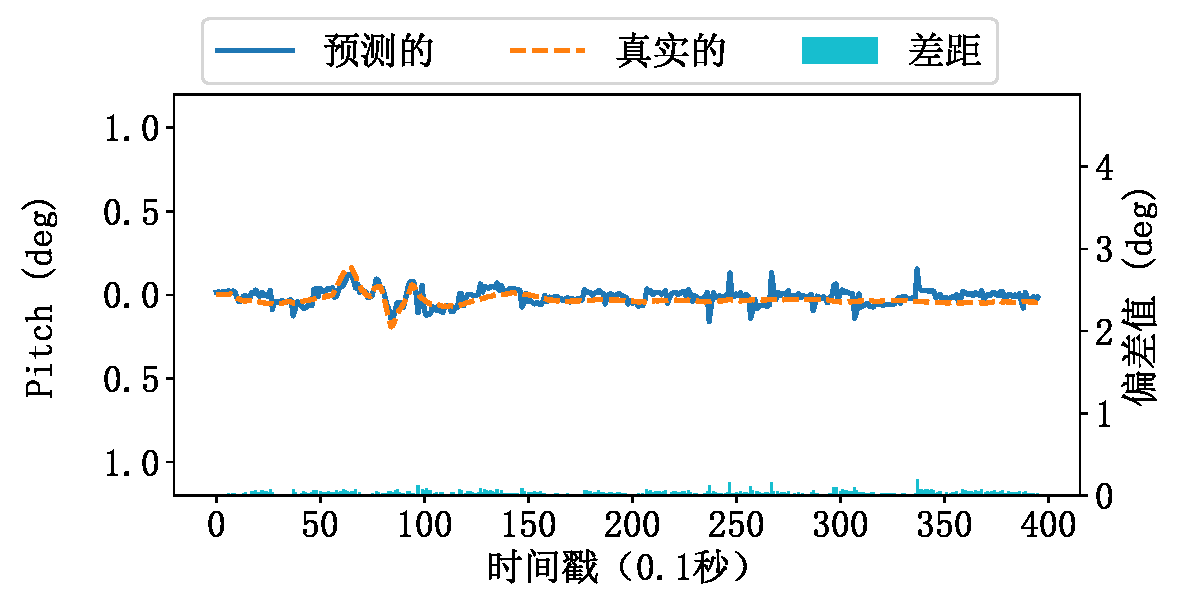
\includegraphics[width=\linewidth]{fig/range/px4_real_pitch.pdf}\quad
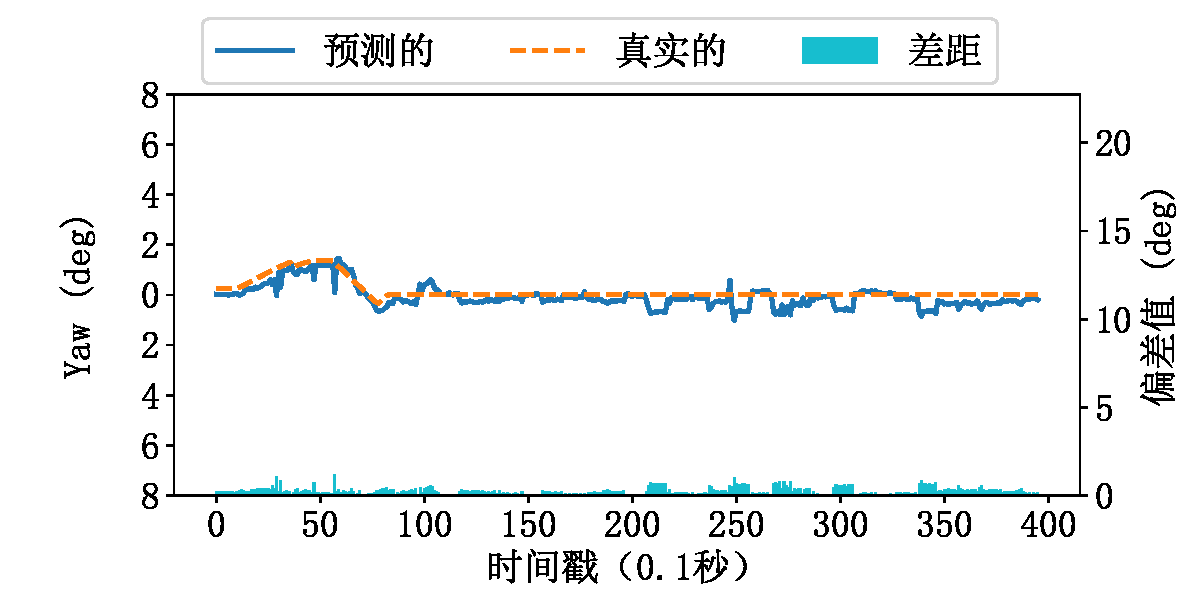
\includegraphics[width=\linewidth]{fig/range/px4_real_yaw.pdf}
\caption{PX4状态变化(Roll, Pitch, 和 Yaw)}
\label{subfig:range_diff2}
\end{minipage}
\end{figure*}

正如前文所述,一个合格的预测器应该能够辅助\icsearcher 准确的区分稳定状态和不稳定状态。
\icsearcher 可以利于预测器来识别更有可能触发不稳定状态的配置从而进模糊测试的迭代过程。
为了证明所生成的预测器的有效性,实验以\tool{Ardupilot}为例,进行了简单阈值分类测试,同时与之前的较为优秀的方法所提出的\tool{LGDFuzzer} 中的预测器进行性能比较。
\tool{LGDFuzzer} 中的预测器是根据预测值和实际值之间的单个偏差来预估配置导致不稳定状态的可能性。
作为对比,本方案中的\icsearcher 则是计算段偏差(段内偏差之和)来做出此确定。

具体来说,此对比实验进行了2,000次飞行测试,其中1,542个由于严重事件而未能完成任务,而458个成功完成任务。
该实验使用2,000个配置中的1,600个(考虑了其中的类别权重)来计算阈值,其余 400 种配置用于测试目的。
当分析包含严重事件(标记为不稳定)的测试日志时,\icsearcher 会提取严重事件时间戳之前发生的片段数据的偏差。
相反,\tool{LGDFuzzer} 仅考虑严重事件时间戳之前发生的单个数据的偏差。
对于不包含严重事件的稳定测试日志(标记为稳定),\icsearcher 随机记录一个段的数据并求其偏差,而 \tool{LGDFuzzer} 随机选择的依旧是单个偏差值。
为了确定阈值,实验计算了稳定 ($ST_{avg}$) 和不稳定 ($UST_{avg}$) 数据的平均分段/单个偏差,然后将阈值设置为这两个平均值之间的中点,即 $(ST_{avg} + UST_{avg}) / 2$。


表~\ref{tab:cross} 显示了通过1600个数据计算出的阈值以及400个测试数据中不稳定的检测性能。
其中片段偏差方案为\icsearcher ,单一偏差方案为 \tool{LGDFuzzer}。
根据表中各自的平均偏差值,片段方案的阈值是3.25,而单一方案的阈值为0.24。
在测试数据中,如果数据超过上述规定的阈值,则被标记为不稳定。

片段偏差方案和单一偏差方案都表明,不稳定状态比稳定状态表现出更大的偏差。
预测器在GA过程中可以利用这一特性来提升模糊测试的效率。
预测器可用通过预测偏差来将配置驱动到更高的偏差值从而诱发不稳定飞行的配置。
与之前未能获得超过 90\% 的 F1-Score的 \tool{LGDFuzzer} 方法相比,\icsearcher 在 F1-Score方面表现更好。
这种改进可归根于片段偏差的使用, 它通过聚合片段内的所有偏差来进行判断,从而减轻了预测器自身准确性的影响,保证了较小的数值波动。
换句话说,在模糊测试中使用片段偏差方法可以更准确地预测某个配置是否会导致不稳定状态。

\begin{table}[ht]
\caption{稳定/不稳定的平均偏差和分类性能}
\label{tab:cross}
\centering
\begin{threeparttable}
\begin{tabular}{c|ccc|ccc}
        \toprule[1.5pt]
        & \makecell*[c]{稳定数据} & \makecell*[c]{不稳定数据}  & 阈值 &
        Precision & Recall & F1-Score \\
        \midrule[0.8pt]

        片段偏差方案 & 1.72 & 4.77 & 3.25 & 92.48\% & 98.19\% & 95.25\% \\

        单一偏差方案 & 0.15 & 0.34 & 0.24 & 80.99\% & 98.19\% & 89.01\% \\
        \bottomrule[1.5pt]
\end{tabular}
\end{threeparttable}
\end{table}

\subsubsection{配置验证}
实验应用测试数据,也就是~\ref{subsec:log_gen} 节中指定的剩余10\%日志数据来进行配置验证实验。
该数据集包括74,074个\tool{Ardupilot}日志条目(总计5,698个片段)和41,096个\tool{PX4}日志条目(总计3,161个片段)。
根据\icsearcher 中的步骤,这些数据被划分为为58和33个簇。
\icsearcher 从每个簇中提取10个样本(如果少于 10 个则为所有可用样本)。
实验总共包含571个片段样本用于测试\tool{Ardupilot},316个片段样本用于测试\tool{PX4}。

随后,实验针对这些样本片段进行模糊搜索,以发掘潜在的错误配置。
对于发现的错误配置,实验再次启动的飞行验证,通过将这些配置上传到无人机并进行飞行以验证是否真的会造成问题。
对于\tool{Ardupilot},\icsearcher 发现了$4,386$个的不重复的潜在不正确配置。
经过模拟器的执行验证,在$4,386$的配置中,有$4,157$被标记为真正不正确的配置,其中分别包括$2,15$个\emph{轨迹偏航}、
$432$\emph{飞行冻结}、
$9$\emph{飞行坠毁}、
$2$\emph{启动后的特权升级}、
和$1,564$\emph{潜在动力损失}。
同样地,对于\tool{PX4},系统发现了$2,282$的潜在不正确配置。
经过验证,$2282$个潜在不正确配置中的$2087$被验证为真正的不正确配置,分别包括$641$\emph{轨迹偏航}、
$228$\emph{飞行冻结}、
$309$\emph{飞行坠毁}、 以及
$909$\emph{启动后的特权升级}。

由于飞控程序设计的原因,两个飞控本身存在差异,例如从传感器驱动程序获取的原始数据、参数列表、飞控算法和日志结构,因此实验结果存在差异。
结果表明,\tool{Ardupilot} 更容易导致轨迹偏差和潜在的推力损失,而 \tool{PX4} 则表现出更高的启动后特权升级和崩溃率。
这是因为\tool{PX4}额外采用了一个模型来检查当前配置是否会导致理论上的最大速度超过阈值,从而决定无人机是否应该起飞。
但是,如果在飞行期间发送这些被曾被拒绝的配置,飞控程序仍然会接收这些配置。
因此,相比\tool{Ardupilot},它导致了更多的启动后权限升级。

\subsection{研究问题2: 适应性}
为了证明系统的灵活范围指南的适应性,本实验利用上一章节已经确认的不正确配置($4,157$个)的结果来生成范围指南。
参照验证结果,灵活的范围指南为\tool{Ardupilot}提供了$178$个\tool{Pareto}解决方案,为\tool{PX4}提供了$213$个\tool{Pareto}解决方案。
每个\tool{Pareto}解决方案代表一个建议的配置范围。
如果范围包含不正确的比例小,可用的数值空间也越小,相应的,也就越安全。
范围包含不正确的比例越大,则可用的数值空间也越大,但是对应的页越危险。

\begin{table}[ht]
\caption{Ardupilot可行范围指南的例子}
\label{tab:range_shrink_cmp}
\centering
\begin{threeparttable}
\begin{tabular}{c|ccc|ccc|ccc}
        \toprule[1.5pt]
          \multirow{2}{*}{参数}  & \multicolumn{3}{c|}{\textit{指南1}} & \multicolumn{3}{c|}{\textit{指南2}} & \multicolumn{3}{c}{\textit{指南3}} \\
         \cmidrule[0.8pt]{2-10}
          ~ & {下界} & 上界 & 减少& {下界} & {上界} & 减少& {下界} & {上界} & 减少 \\
         
         \midrule[0.8pt]
        
        
          PSC\_VELXY\_P  &  0.3 &  5.9   & -5.1\%&  0.3 & 6.0  & -3.3\%  & 0.3 & 6.0   & -3.3\%\\
        
          PSC\_ACCZ\_I  &  0.0 &  2.9   & -3.3\%&  0.0 & 2.4  & -20\%  & 0.0 & 2.6  & -13.3\%\\
        
          ATC\_RAT\_RLL\_P &   0.13 &  0.37   & -51.0\%&  0.125 & 0.375  & -48.9\%  & 0.12 & 0.38  & -46.9\%\\
        
          ATC\_RAT\_RLL\_I &   0.01 &  0.46   & -77.3\%&  0.015 & 0.445  & -78.3.\%  & 0.01 & 0.915  & -54.5\%\\
        
          ATC\_RAT\_PIT\_P &   0.05 &  0.50   & -8.1\%&  0.05 & 0.50  & -8.1\%  & 0.055 & 0.475  & -14.2\%\\
    
          ATC\_ANG\_YAW\_P &   3.1 &  11.9   & -2.2\%&  3.1 & 12.0  & -1.1\%  & 3.0 & 12.0 & -0.0\%\\
        
          WPNAV\_SPEED &   750 &  2000   & -35.8\%&  700 & 2000  & -33.3\%  & 800 & 2000  & -38.4\%\\
         
          ANGLE\_MAX &   1000 &  7020   & -14.0\%&  1000 & 6630  & -19.5\%  & 1000 & 6920 & -15.4\%\\
        % 0, 26, 26; 
        \midrule[0.8pt]
        {$\frac{I}{V}$},{V} & 
        \multicolumn{3}{c|}{0.0\%,26} & 
        \multicolumn{3}{c|}{3.43\%,29} &
         \multicolumn{3}{c}{26.9\%,52} \\
        \bottomrule[1.5pt]
        
\end{tabular}
\begin{tablenotes}
\footnotesize
\item[*] 
\dquote{减少}是相对于原始范围计算的(越小意味着适应性越高),
\dquote{V} 是范围指南涵盖的已验证配置的数量,
\dquote{$\frac{I}{V}$} 是范围指导中错误配置的比例(越小意味着稳定性越高)。
\end{tablenotes}
\end{threeparttable}
\end{table}


\begin{table}[ht]
\caption{PX4可行范围指南的例子}
\label{tab:range_shrink_px4}
\centering
\begin{threeparttable}
\begin{tabular}{c|ccc|ccc|ccc}
        \toprule[1.5pt]
          \multirow{2}{*}{参数}  & \multicolumn{3}{c|}{\textit{指南1}} & \multicolumn{3}{c|}{\textit{指南2}} & \multicolumn{3}{c}{\textit{指南3}} \\
         \cmidrule[0.8pt]{2-10}
          ~ & {下界} & {上界} & 减少& {下界} & {上界} & 减少& {下界} & {上界} & 减少 \\
         
        \midrule[0.8pt]
        
         MC\_ROLL\_P  &  1.0 &  12   & -8.3\%   & 1.4 & 11.9   & -14.1\% &  1.2 & 12.0  & -0.1\%\\
        
          MC\_PITCH\_P  &  0.5 &  12   & -4.1\%   & 3.1 & 12.0  & -4.1\% &  1.8 & 11.9  & -15.8\%\\
        
          MC\_YAW\_P &   1.0 &  5.0   & -20.0\%  & 0.7 & 4.8  & -2.0\% &  0.0 & 4.9  & -2.0\%\\
        
          MPC\_Z\_P &   0.5 &  1.4   & -40.0\%  & 0.0 & 1.4  & -6.7\% &  0.2 & 1.4  & -20.0\%\\
        
          MC\_ROLLRATE\_P &   0.13 &  0.49   & -26.5\%  & 0.08 & 0.50  & -14.2\% &  0.06 & 0.5  & -10.2\%\\
    
          % MPC\_Z\_VEL\_MAX\_DN &   0.9 &  3.3   & -31.4\% & 0.9 & 3.6 & -2.8\% &  0.6 & 3.9  & -5.7\% \\
        
        % 0, 26, 26; 
        \midrule[0.8pt]
        {$\frac{I}{V}$},{V} & 
        \multicolumn{3}{c|}{4.0\%,26} & 
         \multicolumn{3}{c|}{9.3\%,32} & 
         \multicolumn{3}{c}{32.2\%,93} \\
        
        \bottomrule[1.5pt]
\end{tabular}
\begin{tablenotes}
\footnotesize
\item[*] 
\dquote{减少}是相对于原始范围计算的(越小意味着适应性越高),
\dquote{V} 是范围指南涵盖的已验证配置的数量,
\dquote{$\frac{I}{V}$} 是范围指导中错误配置的比例(越小意味着稳定性越高)。
\end{tablenotes}
\end{threeparttable}
\end{table}


表~\ref{tab:range_shrink_cmp} 和 表~\ref{tab:range_shrink_px4}中展示了一些有代表性的\tool{Ardupilot}和 \tool{PX4}的范围样例。
其中\dquote{减少}表示新指南相对于官方指南减少了多少范围(即适应性),减少的越多,适应性越差;
$\frac{I}{V}$表示指南中验证的错误配置的百分比(即稳定性); 越低意味着越安全。
下面对这些样例的其稳定性和适应性的平衡进行分析。
表中分别显示了三个例子,从1到3,它们的稳定性下降,可配置空间(即适应性)增加。
对于\tool{Ardupilot}的配置,\textit{指南1}涵盖了$26$的验证配置。
在这些配置中,只有一个造成了不稳定的状态,这说明稳定性很高。
然而,与原始参数范围相比,这样的范围指南减少了太多,导致适应性低。
与此相反的是,\textit{指南3}实现了高适应性,涵盖了$359$个的被验证的配置,但是其中一半以上(226)是不正确的,这导致了低稳定性。
\textit{指南2}是一个中间选择,涵盖了$52$个被验证的配置,其中只有$38$个是错误的。
同样,对于\tool{PX4}配置,\textit{指南1}是中间选择。它具有最高的安全性,但可用范围最小,它涵盖了$26$个被验证的配置,只有一个是不正确的。
\textit{指南2}和\textit{指南3}分别涵盖了$93$个和$469$个被验证的配置,有$30$个和$346$个的不正确配置。

关于稳定性和适应性的要求,用户可以根据自己的稳定性和适应性要求从\tool{Pareto}方案中自由选择一个合适的范围指南。
如果用户对稳定性有更严格的要求,可以使用较低的误差率范围指南,代价是可配置空间有限。
相反,如果用户有特殊的任务要求(例如,任务是有时间限制的,或者需要一个大的飞行角度来达到目标速度),他们可以考虑牺牲一点稳定性来提高适应性。
例如,如果用户在任务要求中要求参数 \param{MPC\_Z\_P} 为 0.2,则用户可以在\tool{PX4}中选择\textit{指南2}而不是 \textit{指南1}。
尽管\textit{指南2}不是最安全的选项,但其 \param{MPC\_Z\_P}范围 (0.0, 1.4) 优先满足所需值,因此用户可以使用该指南来确定其他参数。


\subsection{研究问题3: 提升}
为了证明该系统的优势,第三个子实验将\icsearcher 与\tool{RVFuzzer}~\cite{rvfuzzer}进行了比较。
\tool{RVFuzzer}利用两种方法\tool{一维变异}和\tool{多维变异}来搜索不正确的配置。
通过使用 \tool{一维变异},以参数的默认值为中心,\tool{RVFuzzer}针对每一个参数分别进行二进制搜索来缩小上下界,直到获得一个不再导致不稳定状态的中点值。
\tool{RVFuzzer}通过\tool{多维变异}来处理多参数同时突变的情况。
与\tool{一维变异}类似,它针对每一个参数都进行一个新的二元突变搜索,但是在这个过程中会引入其他不同参数的极端值(即最大和最小值)。
此外,实验还还比较了\tool{LGDFuzzer}~\cite{han2022control}生成的范围指南。
所有这些实验都基于在\tool{RVFuzzer}使用的六个相同的参数进行对比(见表~\ref{tab:range_cmp_param})。


\begin{table}[ht]
\caption{用于比较的Ardupilot控制程序的参数}
\label{tab:range_cmp_param}
\centering
\begin{tabular}{cccp{0.55\columnwidth}}
        \toprule[1.5pt]
         参数 & 范围 & 默认值 \\
        \midrule[0.8pt]
          PSC\_VELXY\_P & [0.0, 6.0] & $2.0$\\
  
         INS\_POS1\_Z & [-5.0, 5.0] & 0.0\\
        
         INS\_POS2\_Z & [-5.0, 5.0] & 0.0 \\
        
         INS\_POS3\_Z & [-5.0, 5.0] &0.0\\

         WPNAV\_SPEED & [20, 2000] & 500 \\
        
       
         ANGLE\_MAX & [1000, 8000] & 4500\\
        \bottomrule[1.5pt]
\end{tabular}
\end{table}

\subsubsection{搜索遗漏方面的比较}
\tool{RVFuzzer}的最优解仍然存在较多的遗漏情况。
例如,\tool{一维变异}测试中表明参数\param{INS\_POS1\_Z}的正确范围应该保持在$[-4.7, 0.0]$之内,参数官方设定的原始下限为$[-5.0,0.0]$。
然而,在本次实验验证中,在这个范围内仍然有不正确的配置,特别是在$1.0$和$0.0$之间。
在实验分析中,\tool{RVFuzzer}方法的二进制搜索直接跳过了大于$2.5$的值,因为第一个中点(即$2.5$)没有引起不稳定的状态,因此它不会去测试覆盖$[-1.0,0.0]$的空间,导致错误配置的缺失。
而在多参数变异的情况下,实验首先通过\tool{多维变异}确定一个先验的正确范围。
基于这个范围,实验使用\icsearcher 开始另一次搜索来挖掘不正确的配置。
结果表示它仍然检测到$106$个不正确配置。
这样的结果表明,\tool{多维变异}提供的范围有某些缺陷。
从原理的角度分析,\tool{多维变异}仍然是一个一维的变异,因为它使用二进制搜索来分别突变参数,但只导入其他参数的极端值。
它可以被看作是多个一维突变,控制参数之间的关联性有限,因此,它不考虑与范围极值不同的值的影响。
    
\subsubsection{范围指南的比较}
本实验利用\icsearcher 来搜索这六个参数的不正确配置。
结果报告了$1077$个不重复的潜在不正确配置,经过验证,其中$806$个被确定为导致不稳定状态。
随后,\icsearcher 用它们来生成可行的范围指南,并选择了一个样本进行比较。
表~\ref{tab:range_shrink_cmp} 列出了通过四种方法得到的范围,其中\tool{1}是\tool{一维变异}、\tool{M}是\tool{多维变异}、\tool{LGDFuzzer}和\icsearcher 。

\begin{table*}[htb]
\caption{范围指南的对比}
\label{tab:shrink_cmp}
\centering
\begin{threeparttable}
\begin{tabular}{c|cc|cc|cc|cc}
        \toprule[1.5pt]
       \multirow{2}{*}{参数}  &   \multicolumn{2}{c|}{\tool{1}}  &  \multicolumn{2}{c|}{\tool{M}}  & \multicolumn{2}{c|}{LGDFuzzer} & \multicolumn{2}{c}{\icsearcher} \\
        \cmidrule[0.8pt]{2-9}
        ~  &  {下界}  &  {上界}  &  {下界}  &  {上界}  &  {下界}  &  {上界} & {下界}  &  {上界} \\
        \midrule[0.8pt]
         PSC\_VELXY\_P   &  0.1 &  6.0   &  {0.6}  &  6.0  & 1.9 & 4.2 &  0.7  &  4.1 \\
        
        INS\_POS1\_Z   &  -4.7 &  5.0   &   {-1} & 4.1  & -0.5 & 2.1 & -0.7 & 0.8  \\
        
        INS\_POS2\_Z   &  -5.0 &  5.0   &   -0.7 & 3.2  & -0.7 & 1.2 & -0.8 & 0.7 \\
        
        INS\_POS3\_Z   &  -5.0 &  5.0   &   {-0.8} & 3.0  & -0.9 & 3.2 & -0.3 & 0.4 \\
        
        WPNAV\_SPEED   &  50 &  2000   &   {300} & 2000 & 50 & 1950 & 300 & 1950 \\
        
         ANGLE\_MAX   &  1000 &  8000  &   1000 & 8000  & 1100 &4650 &  1000 & 6850  \\
        \midrule[0.8pt]
        {$\frac{I}{V}$},{V} & \multicolumn{2}{c|}{74.8\%,1077} & \multicolumn{2}{c|}{51.4\%,206} & \multicolumn{2}{c|}{28.5\%,14} & \multicolumn{2}{c}{0.0\%,9} \\
        \bottomrule[1.5pt]
\end{tabular}
\begin{tablenotes}
\footnotesize
\item[*]
\tool{1}: 一维变异,
\tool{M}: 多维编译,
\dquote{减少}是相对于原始范围计算的(越小意味着适应性越高),
\dquote{V} 是范围指南涵盖的已验证配置的数量,
\dquote{$\frac{I}{V}$} 是范围指导中错误配置的比例(越小意味着稳定性越高)。
\end{tablenotes}
\end{threeparttable}
\end{table*}


\tool{RVFuzzer}的\tool{1}方法在每个参数范围内获得的减少量很少,因此它不能排除不正确的配置。
\tool{M}避免了一些不正确的配置,但仍然遗漏了其他配置。
\tool{LGDFuzzer}具有更高的安全性,但由于其对潜在错误配置的搜索不如\icsearcher 准确,因此使用相同数据生成的最安全范围不如\icsearcher。
\icsearcher 方法提供了高稳定性,消除了大多数经过验证的错误配置。
其中的一个特殊情况与\param{INS\_POS2\_Z}有关,这个参数的范围由\icsearcher 给出的下限范围小于由\tool{M}给出的范围。
这是因为除开\param{INS\_POS2\_Z},其他参数的范围都较小,因为配置的有效性是根据多个参数而不是单一参数决定的,其他较为严格的参数范围使得\param{INS\_POS2\_Z}可以活动更大的可配置空间。

\param{ANGLE\_MAX}影响飞行倾角,在使用过程中主要用于姿态调整,过大的值不适合姿势调整。
\param{WPNAV\_SPEED}的数值太小会使无人机更容易冻结,因此\tool{M}和\icsearcher 都减少了这个参数的下界范围。
\icsearcher 返回的 \param{INS\_POS*\_Z}的范围比\tool{M}提供的范围小,前者更接近于默认值。
事实上,改变\param{INS\_POS*\_Z}会影响惯性测量单元的位置判断。
在实际应用中,这些参数不应该与默认值有太大的偏差。
\param{PSC\_VELXY\_P}影响了系统对加速度的输出增益,过大的增益容易造成无人机的偏差或推力损失。
    
\subsubsection{时间消耗的比较}
此处分析了 \icsearcher、\tool{LGDFuzzer}和\tool{RVFuzzer}所花费的时间,表~\ref{tab:range_time} 所示。
\icsearcher 和 \tool{LGDFuzzer} 应用了相同的数据,启动了多次模拟并花费了696秒的时间来收集飞行日志。
在预测器生成阶段,\icsearcher 花费了$703$秒,\tool{LGDFuzzer} 花费了$700$秒来训练预测器直到达到收敛。
然后,\icsearcher 和\tool{LGDFuzzer}的搜索器分别花费了 $244$ 和 $156$ 秒进行迭代。
通过六线程验证(\tool{RVFuzzer}由于其二分搜索而无法使用多线程),它们分别花费了$35$和$33$分钟。
不同之处在于,\icsearcher 搜索到的潜在错误配置中有 94.7\% 被确认为正确,而\tool{LGDFuzzer}为 84.7\%,换句话说,在近似耗时的情况下,\icsearcher 比\tool{LGDFuzzer}更准确。
最终,\icsearcher 花费了$50$分钟,\tool{LGDFuzzer} 花费了$47$分钟。
值得注意的是,数据标记和预测器生成是一次性成本。
相比之下,根据配置的不同,\tool{RVFuzzer}需要20到120秒来完成一次飞行测试任务。
在实验中,\tool{RVFuzzer}花费了 $126$ 分钟来生成六个参数的指导方针。
而如果参数数量增加,计算复杂度将会增加。
\icsearcher 的时间消耗仍然接近于使用六个参数的时间消耗,因为预测器所需的时间基本保持不变。

\begin{table}[ht]
\small
\caption{不同工具的时间消耗}
\label{tab:range_time}
\centering
\begin{tabular}{c|ccccc}
        \toprule[1.5pt]
         
         
         \multirow{2}{*}{工具} & \multirow{2}{*}{预训练} & \multirow{2}{*}{搜素} & 验证  & \multirow{2}{*}{总计} \\
         & & & (6线程) & \\
        \midrule[0.8pt]
          RVFuzzer & - & 126分钟 & - & 126分钟 \\
  
          LGDFuzzer & 700秒 & 156秒 & 33分钟 &  47分钟 \\

          \icsearcher & 703秒 & 241秒 & 35分钟 &  50分钟  \\
        
        \bottomrule[1.5pt]
\end{tabular}
\end{table}


\subsection{样例研究}
该章节选择了几个有代表性的例子来详尽展示这些不正确配置造成的飞行轨迹。

\begin{itemize}
    \item \textbf{轨迹偏航:} 在的实验中,有两种主要的偏差情况,过冲和远飞。
    当从一个航点飞到另一个航点时。 
    无人机首先加速以达到目标速度,在接近下一个航点时减速。
    如果配置设置不当, 无人机在接近航点的时候无法降低速度。
    这就造成了过冲偏偏差(无人机无法及时刹停)。
    相比之下,远飞就危险多了,因为无人机不断偏离其任务计划的路径。
    实验中利用一个真实的无人机实验来证明这些不稳定状态造成的损害。
    该实验设置了一个简单的环绕飞行任务和一个无人机配置,该配置在模拟测试中,导致了飞离的偏差。
    在某一实验中,在装载了该配置后,无人机偏离了任务计划的路径, 不幸的是,尽管实验中用RC控制器(远程手动控制器)将其模式手动切换到\tool{land},以稳定无人机并尝试让其降落。
    无人机仍然无法稳定,并不断地偏离。
    在检查了离线飞行记录后,当手动切换到\tool{land}模式时,系统报告了一个切换错误,表明它不能稳定和降落。
    换句话说,如果不及时处理不正确的配置,飞行稳定性甚至不能被手动纠正。
    
    \item \textbf{飞行冻结:}
    飞行冻结主要有两种情况。
    一个不正确的增益参数限制了飞行速度,使其无法达到预期的位置,或者影响了飞行位置,导致无人机在小范围内绕飞。 
    实验中采用真实的无人机体验测试了环绕飞行的情况,无人机一直在盘旋,无法完成既定的任务。
    它的离线飞行日志显示,无人机一直在 \tool{althold}(盘旋飞行)和 \tool{land}模式之间切换飞行。
    
    \item \textbf{飞行坠毁:}
    无人机坠毁的原因可能是起飞时翻滚或因下降速度不当而撞到地面,实验中的案例显示了无人机起飞后直接造成了侧翻。

    \item \textbf{潜在动力损失:}
    这种情况主要是由角度或速度的过度变化引起的。
    飞行控制器试图将其位置恢复到正常,但电机的功率不能满足要求。
    在恢复推力损失或稳定高度方面的失败将导致无人机坠毁。
    在事后分析中发现,改变与惯性测量单元位置(如:\param{INS\_POS*\_Z})和PID角度控制器(如:\param{ATC\_ANG\_*\_P/I/D})相关的控制参数可以迫使无人机进入一个逐渐放大的振荡。
    
    \item \textbf{启动后的特权升级:}
    启动后的权限升级是本解决方案新定义的一种错误类型。
    一个控制程序通常包含一个检查机制来防止配置中的明显错误。
    如果参数与位置控制器有关(例如,\param{ATC\_*\_*\_P/I/D}),当地面站试图解锁无人机时,不正确的配置会引起警告。
    但事实上,如果使用者在无人机起飞后更新配置,控制系统仍然接受它。
    这最终促使无人机变得不稳定和失去控制。
\end{itemize}


\section{本章小结}
无人机控制参数的不正确配置。由合法用户设置的或由攻击者发送的不合时宜的配置参数,会破坏无人机的飞行状态,影响无人机飞行任务的完成。
本节引入了一种基于基于学习引导的模糊分析系统,可以有效地检测出官方引导范围中的潜在不正确的参数配置。
该系统使用 一种以机器学习为指导的模糊处理方法,结合机器学习所构建的预测器,测试发掘会影响无人机飞行的配置。
本节实验还与其他先进工具进行比较,实验结果表明,\icsearcher 在各个方面都表现出较强的性能。
尽管该方法是为空中无人机设计的,其方法也可以用于其他具有复杂控制的移动设备,如水下无人机。
